%%%%%%%%%% *** The Title %%%%%%%%%%
\title[]{뇌우와 토네이도\\\small{제10장}}

\begin{frame}[plain] %title page
	\titlepage
\end{frame}


\section{명칭의 의미}


\begin{frame}[t]{Cyclone}
	\begin{tabular}{ll}
		\begin{minipage}[t]{0.45\textwidth}\scriptsize
			\begin{figure}[t]
				\includegraphics[trim=50 210 280 230, clip, page=299, width=\textwidth]{\bookfile}
			\end{figure}
		\end{minipage}	
		&
		\begin{minipage}[t]{0.5\textwidth} \scriptsize	
			\questionset{사이클론 용어가 사용되는 세가지에 대해 기술하시오.}
			\solutionset{1) 저기압 중심 주변의 회전을 의미함(규모나 강도와 무관함)\\			
			2) 인도양에서는 그 지역에서의 허리케인\\			
			3) 일부 지역에서는 토네이도를 사이클론으로 부름 \newline}
			
			\questionset{중위도 저기압, 토네이도, 허리케인의 풍속과 규모를 비교하시오.}
			\solutionset{토네이도가 가장 작고, 지속 시간도 가장 짧다. 하지만 가장 강한 바람을 형성한다.\\
				중위도 저기압은 셋 중 가장 크지만, 상대적으로 약한 바람을 가진다.\\
			허리케인(평균 지름 $600\rm{~km}$)은 토네이도(지름 $0.25\rm{~km}$) 보다 크고, 지속시간도 길지만 중위도 저기압(지름 $1600 \rm{~km}$) 보다는 작다. 풍속은 적어도 $119 \rm{~km/h}$이다.}
						
		\end{minipage}
	\end{tabular}
\end{frame}




\section{뇌우}


\begin{frame}[t]{뇌우}
	\begin{tabular}{ll}
		\begin{minipage}[t]{0.45\textwidth}\scriptsize
			뇌우 : 번개와 천둥을 생성하는 폭풍우\\
			천둥, 번개, 바람, 우박을 동반하는 경우가 많음\\
			공기의 강력한 상하 움직임\\
			
			가변적 특성 : 독자적으로 생기기도 하며, 사이클론과 연관되어 생기기도 함\\
			중위도 저기압의 한랭 전선을 따라 뇌우가 형성되기도 하며, 허리케인은 뇌우 활동을 넓게 확대
			
		\end{minipage}	
		&
		\begin{minipage}[t]{0.5\textwidth} \scriptsize	
			뇌우의 종류\\
			기단 뇌우: mT 기단과 같은 따뜻하고 습한 공기가 불안정한 환경에서 상승하여 적란운을 형성. \\
			위험 뇌우: 풍속이 매우 빠르고, 우박과 홍수, 토네이도를 형성 
			지표의 불균등 가열, 전선면에서의 상승, 수렴대에서 형성
			
		\end{minipage}
	\end{tabular}
\end{frame}



\begin{frame}[t]{뇌우}
	\begin{tabular}{ll}
		\begin{minipage}[t]{0.5\textwidth}\scriptsize
			\begin{figure}[t]
				\includegraphics[trim=30 470 245 50, clip, page=300, width=\textwidth]{\bookfile}
			\end{figure}
		\end{minipage}	
		&
		\begin{minipage}[t]{0.45\textwidth} 
			\begin{figure}[t]
				\includegraphics[trim=270 30 50 520, clip, page=300, width=\textwidth]{\bookfile}
			\end{figure}
			
		\end{minipage}
	\end{tabular}
	\newline


	\questionset{뇌우가 가장 빈번한 곳은 지구 전체에서, 미국에서 어디일까?}
	\solutionset{지구 전체: 적도 수렴대와 관련된 수렴과 따뜻하고, 습하고, 불안정한 공기 덩이가 조화를 이루는 열대 지방\\
		미국: 멕시코만과 플로리다 지역이 가장 활발}

\end{frame}






\begin{frame}[t]{뇌우}
	\begin{tabular}{ll}
		\begin{minipage}[t]{0.45\textwidth}\scriptsize
			\begin{figure}[t]
				\includegraphics[trim=320 450 50 50, clip, page=301, width=\textwidth]{\bookfile}
			\end{figure}
		\end{minipage}	
		&
		\begin{minipage}[t]{0.5\textwidth} \scriptsize	
			\questionset{미래에 로키 산맥 동쪽과 미국의 동부, 남부의 위험 뇌우 활동은 어떻게 변화하겠는가?}
			\solutionset{정교한 기후 모형을 통한 뇌우 활동의 예측 결과를 보면 로키 산맥 동쪽은 위험 뇌우 활동이 줄어들고, 미국 동부, 남부 지역은 위험 뇌우 활동이 증가할 것으로 보인다. \newline}
	
			\questionset{뇌우 형성의 최우선 조건은 무엇인가?}
			\solutionset{따뜻하고, 습하고, 불안정한 공기가 필요하다. 부가적으로 공기가 상승할 수 있도록 하는 기작이 필요하다. \newline}
			
			\questionset{뇌우가 가장 활발한 계절과 시간은 언제인가? 이유와 함께 설명하시오.}
			\solutionset{공기의 불안정성을 증가시키는 지표 가열이 가장 강한 여름철 오후가 뇌우 생성이 가장 활발함.}
			
		\end{minipage}
	\end{tabular}
\end{frame}






\section{기단 뇌우}



\begin{frame}[t]{기단 뇌우 (air-mass thunderstorms)}
	\begin{tabular}{ll}
		\begin{minipage}[t]{0.6\textwidth}\scriptsize
			\begin{figure}[t]
				\includegraphics[trim=50 480 220 50, clip, page=302, width=\textwidth]{\bookfile}
			\end{figure}
		\end{minipage}	
		&
		\begin{minipage}[t]{0.35\textwidth} \scriptsize	
			\questionset{기단 뇌우가 형성되는 과정을 세 단계로 설명하시오.}
			\solutionset{1) 적운 단계에서는 따뜻하고 습한 상승 기류가 대부분이고, 수증기가 응결하여 적란운을 형성\\
			2) 성숙 단계에서는 강수가 형성되고, 차가운 하강 기류도 존재한다. 뇌우의 강도가 최고이며, 천둥, 번개, 우박 등을 동반\\
			3) 소멸 단계에서는 하강 기류가 대부분이고 하강 기류의 냉각효과로 인해 뇌우를 유지시키는 따뜻하고 습한 상승 기류가 끝남.}
		
		\end{minipage}
	\end{tabular}
\end{frame}




\begin{frame}[t]{적운 단계(cumulus stage)}
	\begin{tabular}{ll}
		\begin{minipage}[t]{0.65\textwidth}\scriptsize
			\begin{figure}[t]
				\includegraphics[trim=0 0 0 550, clip, page=302, width=\textwidth]{\bookfile}
			\end{figure}
		\end{minipage}	
		&
		\begin{minipage}[t]{0.3\textwidth} \scriptsize	
			\begin{figure}[t]
				\includegraphics[trim=80 560 474 50, clip, page=302, width=0.8\textwidth]{\bookfile}
			\end{figure}
			
		\end{minipage}
	\end{tabular}
	\scriptsize 

	지표의 불균등 가열에 의해 생성, 공기의 상승류로 이어짐\\
	부양하는 열기포가 갠날 적운을 형성 (왼 그림)\\
	갠날 적운의 증발로 습윤한 공기가 공급되며, 습기가 충분해지면 구름이 증발하지 않고 계속 연직(수직운)으로 발달(오른 그림)
\end{frame}




\begin{frame}[t]{성숙 단계(mature stage)}
	\begin{tabular}{ll}
		\begin{minipage}[t]{0.3\textwidth}\scriptsize
			\begin{figure}[t]
				\includegraphics[trim=200 560 358 50, clip, page=302, width=0.8\textwidth]{\bookfile}
			\end{figure}
			
		\end{minipage}	
		&
		\begin{minipage}[t]{0.65\textwidth} \scriptsize	
			결빙 고도 위까지 구름이 발달하면 Bergeron 과정에 의해 강수 발생. \\
			구름 내부 강수의 누적으로 상승 기류가 강수를 지지하기 어려워 짐.\\
			강수가 공기와 함께 하강하여 하강 기류 시작. \\
			주변 한랭 건조 공기가 구름 안으로 유입(entrainment)되면 하강 기류 강화\\
			하강 기류가 구름 밑면을 떠나 강수가 방출되면 ‘성숙 단계’ 시작\\
			상승 기류와 하강 기류가 나란히 존재하며 구름을 계속 성장시킴\\
			뇌우 발달단계에서 가장 활발한 시기이며, 돌풍, 번개, 폭우가 발생하고 때론 작은 우박이 동반되기도 함\\
									
			\questionset{유입이 뇌우의 하강 기류를 강화하는 이유는 무엇인가?}
			\solutionset{유입 과정에서 추가된 공기는 건조하기에 상대적으로 무거워서 하강 기류를 강화한다. 유입된 건조 공기는 낙하하는 물방울을 증발시키고, 증발 냉각으로 인해 하강 기류는 더욱 냉각되어 강화된다.}
			
		\end{minipage}
	\end{tabular}
\end{frame}



\begin{frame}[t]{소멸 단계(dissipating stage)}
	\begin{tabular}{ll}
		\begin{minipage}[t]{0.3\textwidth}\scriptsize
		\begin{figure}[t]
			\includegraphics[trim=317 560 248 50, clip, page=302, width=0.8\textwidth]{\bookfile}
		\end{figure}
		\end{minipage}	
		&
		\begin{minipage}[t]{0.65\textwidth} \scriptsize	
			하강 기류가 시작되면 주변의 한랭 건조 공기가 더 많이 유입되어 구름 전체를 하강 기류가 지배\\
			강수의 냉각효과와 상층의 차가운 공기 유입으로 인해 상승 기류를 통한 습기 공급이 중단되어 구름이 증발됨\\
			기단 뇌우 내의 응결된 수증기의 80\%가 다시 대기로 증발\\
			
			\questionset{기단 뇌우의 수명이 짧은 이유는 무엇인가?}
			\solutionset{하강 기류가 기단 뇌우를 지속시키는 수분 공급을 차단시켜 스스로 사라지게 만든다.}
			
		\end{minipage}
	\end{tabular}
\end{frame}







\section{위험 뇌우}


\begin{frame}[t]{위험 뇌우(Severe thunderstorms)}
	\begin{tabular}{ll}
		\begin{minipage}[t]{0.4\textwidth}\scriptsize
			\begin{figure}[t]
				\includegraphics[trim=50 400 330 50, clip, page=304, width=\textwidth]{\bookfile}
			\end{figure}
		\end{minipage}	
		&
		\begin{minipage}[t]{0.55\textwidth} \scriptsize	
			위험 뇌우는 풍속이 $93 \rm{~km/h}$ 이상이거나, 지름 $2.5 \rm{~cm}$ 이상의 우박을 동반하거나, 토네이도 생성하는 경우를 말한다.\\
			미국에서 발생하는 연간 10만 여 개의 뇌우 가운데 $10\%$ 가량 위험 뇌우에 도달함. \\
		
			\questionset{일부 뇌우의 수명이 기단 뇌우보다 긴 이유는 무엇인가?}
			\solutionset{연직 바람 시어. 즉, 서로 다른 고도에서의 풍향과 풍속의 변화 때문이다.\\
				이런 조건에서는 상승 기류가 연직 상태를 유지하지 못하고 기울어져서 구름 내부 상층에서 형성된 강수가 상승 기류가 아닌 하강 기류 속으로 떨어진다. 
				구름 아래에서는 밀도가 더 크고 한랭한 하강기류가 지면을 따라 퍼진다. 유출되는 하강기류의 전방 경계는 습윤한 지상 공기를 구름속으로 밀어넣는다. 
				이로 인해 상승 기류가 계속 유지되고, 구름이 성층권 하부까지 올라가기도 하는데 이를 돌출 꼭대기(overshooting top) 이라고 한다.}
						
		\end{minipage}
	\end{tabular}
\end{frame}




\begin{frame}[t]{위험 뇌우(Severe Thunderstorms)}
	\begin{tabular}{ll}
		\begin{minipage}[t]{0.45\textwidth}\scriptsize
			\begin{figure}[t]
				\includegraphics[trim=50 400 330 50, clip, page=304, width=\textwidth]{\bookfile}
			\end{figure}
		\end{minipage}	
		&
		\begin{minipage}[t]{0.5\textwidth} \scriptsize	
			적란운 하부에는 밀도가 높은 한랭한 공기가 지면을 따라 퍼져 나가, 이 하강 기류의 전방 경계는 쐐기의 역할을 하여 온난 습윤한 지표 공기를 뇌우 속으로 밀어넣음\\
			이를 통해 하강 기류가 상승 기류를 유지하는 역할을 하여 뇌우를 지속시킴\\


			\questionset{돌풍 전선(미니 한랭 전선)이란 무엇인지 설명하시오.}
			\solutionset{돌풍 전선은 하강하는 차가운 공기가 주변의 온난한 공기 속으로 전진하며 형성되는 미니 한랭 전선을 돌풍 전선이라고 함. }
			
		\end{minipage}
	\end{tabular}
\end{frame}




\begin{frame}[t]{두루마리 구름}
	\begin{tabular}{ll}
		\begin{minipage}[t]{0.4\textwidth}\scriptsize
			\begin{figure}[t]
				\includegraphics[trim=350 50 30 470, clip, page=304, width=\textwidth]{\bookfile}
			\end{figure}
		
		\end{minipage}	
		&
		\begin{minipage}[t]{0.55\textwidth} \scriptsize	
			돌풍 전선이 이동함에 따라 강한 난류가 먼지와 흙을 끌어 올려 전진하는 경계가 눈에 보이게 되는데, 이때 두루마리 구름이 형성되기도 한다.
			\\

			\questionset{위험 뇌우 안의 하강 기류가 상승 기류를 유지하기 위한 역할은 무엇인가?}
			\solutionset{위험 뇌우에서 하강 기류는 지표면을 따라 흩어지고, 따뜻하고 습한 지표면의 공기를 파고들어 이 공기가 위험 뇌우로 들어오게 하여 따뜻한 공기의 상승을 유지함. \newline}
			
			\questionset{위험 뇌우가 발달하는 과정을 돌풍 전선의 역할과 관련지어 서술하시오}
			\solutionset{적란운 하부에는 밀도가 높은 한랭한 공기가 지면을 따라 퍼져 나가, 이 하강 기류의 전방 경계에 형성된 돌풍 전선이 쐐기의 역할을 하여 온난 습윤한 지표 공기를 뇌우 속으로 밀어 넣어 이를 통해 하강 기류가 상승 기류를 유지하는 역할을 하여 뇌우를 발달시킨다.}
			
			
		\end{minipage}
	\end{tabular}
\end{frame}




\begin{frame}[t]{거대 세포 뇌우 (Supercell thunderstorms)}
	\begin{tabular}{ll}
		\begin{minipage}[t]{0.55\textwidth}\scriptsize
			\begin{figure}[t]
				\includegraphics[trim=40 380 50 50, clip, page=305, width=\textwidth]{\bookfile}
			\end{figure}
		\end{minipage}	
		&
		\begin{minipage}[t]{0.4\textwidth} \scriptsize	
			매우 위험한 기상을 유발함
			높이가 $20 \rm{~km}$가 넘는 하나의 강력한 단일 세포이며 직경은 $20 \sim 50 \rm{~km}$\\
			
			Mesocyclone(중규모 저기압)\\
			초대형 세포 뇌우 안에서 저기압성으로 회전하는 공기 기둥\\
			저기압성으로 회전하는 공기 기둥이 연직 쉬어에 의해 수직으로 비틀어져 형성
			토네이도가 종종 형성
						
		\end{minipage}
	\end{tabular}
\end{frame}






\begin{frame}[t]{마개 역전(capping inversion)}
	\begin{tabular}{ll}
		\begin{minipage}[t]{0.9\textwidth}\scriptsize
			\begin{figure}[t]
				\includegraphics[trim=50 50 50 550, clip, page=305, width=\textwidth]{\bookfile}
			\end{figure}
		\end{minipage}	
		&
		\begin{minipage}[t]{0.05\textwidth} \scriptsize	
			
		\end{minipage}
	\end{tabular} 
	
	\questionset{거대 세포를 지속시키기 위해 필요한 잠열을 얻을 수 있게 하는 조건은 무엇이며, 어떤 과정으로 조건을 만족시키는가?}
	\solutionset{잠열을 얻기 위해서는 대류권 하부를 온난하고 매우 습윤하게 유지해야 함. 지상 수 킬로미터 위에 형성된 역전층이 이러한 요건을 마련해 줌. 역전층은 공기 혼합을 막아 지표 가열이 역전층 아래의 온도와 습도를 높여주고, 결국 아래로부터의 강한 혼합으로 역전층이 국지적 쇠퇴함. 이러한 불안정한 공기는 폭발적으로 분출하여 유별나게 큰 적란운 탑을 생성하고, 여기에 집중적이고 지속적 상승 기류가 더해져 거대 세포가 형성.}

\end{frame}



%\begin{frame}[t]{다 세포 뇌우}
%	\begin{tabular}{ll}
%		\begin{minipage}[t]{0.45\textwidth}\scriptsize
%			\begin{figure}[t]
%				\includegraphics[trim=50 290 50 50, clip, page=218, width=\textwidth]{\bookfile}
%			\end{figure}
%		\end{minipage}	
%		&
%		\begin{minipage}[t]{0.5\textwidth} \scriptsize	
%			돌풍 전선이 이동하며 강제상승을 유발하여 새로운 뇌우를 형성시키기도 함
%			(다세포 뇌우) 
%			각 세포는 일반 뇌우(단세포 뇌우)의 특성을 보임
%			
%			- 각 세포는 풍향을 따라 이동
%			- 다세포 뇌우는 전체적으로 풍향의 오른쪽 방향으로 진행
%			- (이 경우) 다세포 뇌우의 오른쪽 끝은 새로운 뇌우 발생, 왼쪽 끝은 소멸하는 뇌우 위치
%			
%			
%		\end{minipage}
%	\end{tabular}
%\end{frame}



\begin{frame}[t]{스콜선(Squall lines)}
	\begin{tabular}{ll}
		\begin{minipage}[t]{0.4\textwidth}\scriptsize
			\begin{figure}[t]
				\includegraphics[trim=50 550 350 0, clip, page=306, width=\textwidth]{\bookfile}
			\end{figure}
		\end{minipage}	
		&
		\begin{minipage}[t]{0.55\textwidth} \scriptsize	
			스콜선 : 뇌우가 비교적 좁은 띠 형태로 이루어진 것\\
			온난 건조한 대륙성 열대 기단이 중위도 저기압의 온난역을 밀면서 한랭 전선 앞쪽 $100 \sim 300 \rm{~km}$에서 발달하며, 유방 구름 하늘이 스콜선 앞에 나타남.\\
			대부분의 스콜선은 한랭 전선을 따라 발생한 강한 상승으로 만들어진 것이 아니며, 일부는 지표의 온난 습윤한 공기와 활발한 상층 제트류의 결합으로 생성.\\
			스콜선은 제트류로 인한 발산과 그에 따른 상승이 남쪽에서 강하고 지속적으로 유입된 온난 습윤한 하층류와 만날 때 형성 \\
			수증기량이 급변하는 건조 전선을 따라 자주 발생함.
			
			
		\end{minipage}
	\end{tabular}
\end{frame}



\begin{frame}[t]{스콜선(Squall lines)}
	\begin{tabular}{ll}
		\begin{minipage}[t]{0.6\textwidth}\scriptsize
			\begin{figure}[t]
				\includegraphics[trim=50 0 350 550, clip, page=306, width=0.49\textwidth]{\bookfile}
				\includegraphics[trim=350 375 50 50, clip, page=306, width=0.49\textwidth]{\bookfile}
			\end{figure}
		\end{minipage}	
		&
		\begin{minipage}[t]{0.35\textwidth} \scriptsize	
			\questionset{건조 전선을 따라 스콜선이 형성되는 과정을 설명하시오.}
			\solutionset{건조 전선은 습도가 갑작스럽게 변하는 좁은 경계 영역으로, cT기단이 중위도 저기압의 한랭 전선 앞의 온난역을 밀 때 건조 전선을 따라 형성된다. 스콜선은 무거운 cT기단이 상대적으로 가벼운 mT 기단을 강제적으로 상승시킬 때 형성됨.}
			
		\end{minipage}
	\end{tabular}
\end{frame}



\begin{frame}[t]{중규모 대류 복합체}
	\begin{tabular}{ll}
		\begin{minipage}[t]{0.55\textwidth}\scriptsize
			\begin{figure}[t]
				\includegraphics[trim=350 50 50 550, clip, page=307, width=\textwidth]{\bookfile}
			\end{figure}
		\end{minipage}	
		&
		\begin{minipage}[t]{0.4\textwidth} \scriptsize	
			중규모 대류 복합체 (Mesoscale convective complexes, MCC)는 타원형 내지 원형 무리로 구성된 많은 수의 개별 뇌우로 구성됨.\\
			최소 $100,000 \rm~{km^2}$ 의 영역을 뒤덮음.\\
			보통 느리게 이동하여 12시간 이상 지속되며, 보통 미국의 대평원에서 형성되는 경향이 있음.\\는
			악기상을 동반하기만 농업지대에 상당향의 강우를 제공하는 유익한 측면도 있음.
			
		\end{minipage}
	\end{tabular}
\end{frame}



\begin{frame}[t]{돌발 홍수}
	\begin{tabular}{ll}
		\begin{minipage}[t]{0.9\textwidth}\scriptsize
			\begin{figure}[t]
				\includegraphics[trim=350 480 50 110, clip, page=307, width=0.49\textwidth]{\bookfile}
				\includegraphics[trim=350 480 50 110, clip, page=308, width=0.49\textwidth]{\bookfile}
			\end{figure}
		\end{minipage}	
		&
		\begin{minipage}[t]{0.05\textwidth} \scriptsize	
			
		\end{minipage}
	\end{tabular}
	\scriptsize 
	\newline
		
	짧은 시간 동안 많은 양의 비를 내리는 국지적 홍수로 가파른 비탈로 인해 빗물이 좁은 계곡으로 빨리 흘러갈 수 있는 산악 지대에서 흔히 발생.

\end{frame}


\begin{frame}[t]{돌발 홍수}
	\begin{tabular}{ll}
		\begin{minipage}[t]{0.45\textwidth}\scriptsize
			\begin{figure}[t]
				\includegraphics[trim=50 280 320 335, clip, page=308, width=\textwidth]{\bookfile}
			\end{figure}
		\end{minipage}	
		&
		\begin{minipage}[t]{0.5\textwidth} \scriptsize	
			\questionset{머셔 크리크가 뉴오컨 크리크에 비해 시단 당 단위 면적 유출량이 급격히 증가하는 이유는 무엇인가?}
			\solutionset{도시 지역은 불투수성 지면 비율이 높아 호우에 따른 유출이 빠르기 때문에 돌발 홍수에 취약하다.}
			
		\end{minipage}
	\end{tabular}
\end{frame}




\section{번개와 천둥}



\begin{frame}[t]{번개(lightening)}
	\begin{tabular}{ll}
		\begin{minipage}[t]{0.4\textwidth}\scriptsize
			\begin{figure}[t]
				\includegraphics[trim=320 280 50 120, clip, page=309, width=\textwidth]{\bookfile}
			\end{figure}
		\end{minipage}	
		&
		\begin{minipage}[t]{0.55\textwidth} \scriptsize	
			\begin{figure}[t]
				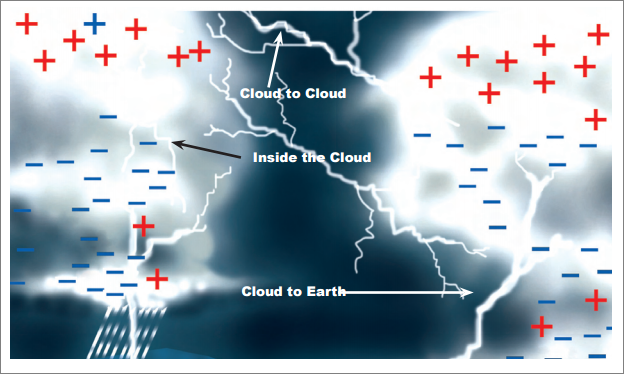
\includegraphics[width=0.8\textwidth]{./images/cheatsheet_24221.png}
			\end{figure}

			\begin{itemize}
				\item 거대한 적란운 발생시 전하 분리가 일어나면 구름의 일부는 양전하, 음전하를 띠게 됨.
				\item 약 80 \%는 구름 내부 또는 구름과 구름 사이에 방전이 일어남. 
				\item 약 20 \%는 구름과 지면 사이의 전하 차이로 인해 방전되며 번개 형성
				\item 구름은 강절연에(약전도체)이기 때문에 번개가 발생하기 전에 전위가 매우 높아야 함.
			\end{itemize}

		\end{minipage}
	\end{tabular}
\end{frame}



\begin{frame}[t]{번개(lightening)}
	\begin{tabular}{ll}
		\begin{minipage}[t]{0.5\textwidth}\scriptsize
			\begin{figure}[t]
				\includegraphics[trim=40 30 350 520, clip, page=309, width=\textwidth]{\bookfile}
			\end{figure}
		\end{minipage}	
		&
		\begin{minipage}[t]{0.45\textwidth} \scriptsize	
			\questionset{미국 내에서 번개에 의한 사망자 수는 얼마나 많은가?}
			\solutionset{미국 내에서 폭풍우 관련 사망 원인 가운데 홍수에 이어 두번째로 번개 사망 수치가 많다. 매년 100명이 사망하고, 1000명 이상이 상해를 입는다. }
			
			
		\end{minipage}
	\end{tabular}
\end{frame}



\begin{frame}[t]{섬광과 뇌격}
	\begin{tabular}{ll}
		\begin{minipage}[t]{0.35\textwidth}\scriptsize
			\begin{figure}[t]
				\includegraphics[trim=50 55 350 410, clip, page=312, width=\textwidth]{\bookfile}
			\end{figure}
		\end{minipage}	
		&
		\begin{minipage}[t]{0.55\textwidth} \scriptsize	
			
			\begin{figure}[t]
				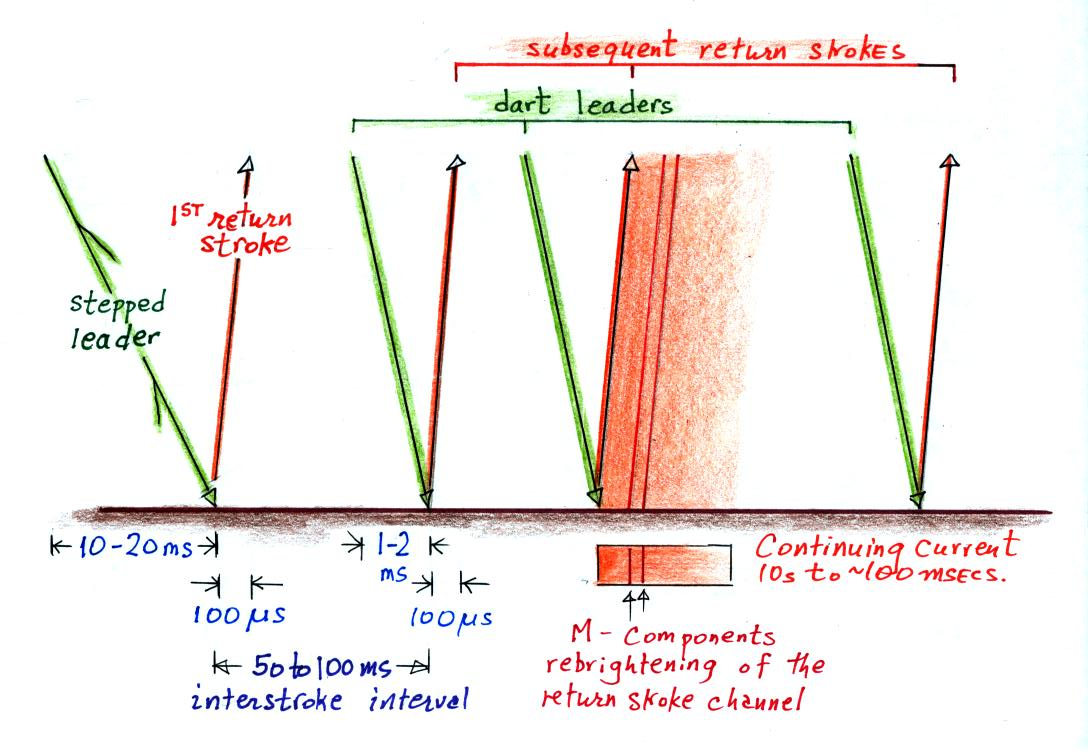
\includegraphics[width=0.8\textwidth]{./images/4stroke_flash.jpg}
			\end{figure}

		섬광(flash): 몇 십분의 1초 동안 광선 형태로 나타나는 총 방전\\
		뇌격(stroke): 섬광을 구성하는 개별 요소 (뇌격은 아래로 전파되는 선도로 이루어짐)\\
		되돌이 뇌격(return stroke): 도전로 하단에 있던 전자가 지면 쪽으로 이동하면서 경로 위쪽에 자리잡고 있던 전자가 아래로 이동. 전자 흐름의 통로가 계속 위로 확대되기 때문에 동반하는 방전 (경로 내의 음전하가 지면으로 이동)\\	
		\end{minipage}
	\end{tabular}
\end{frame}




\begin{frame}[t]{선도}
	\begin{tabular}{ll}
		\begin{minipage}[t]{0.475\textwidth}\scriptsize
			\begin{figure}[t]
				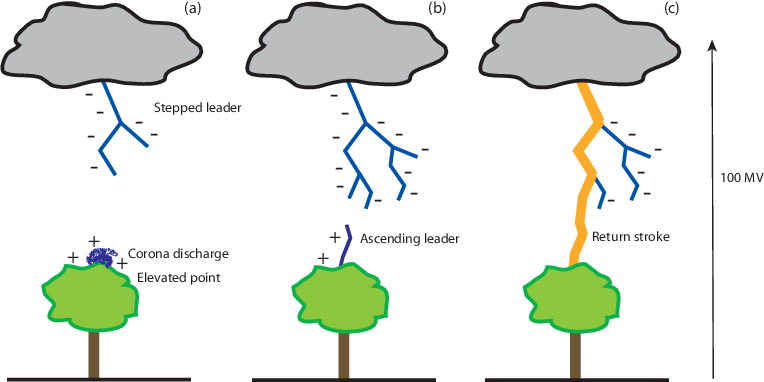
\includegraphics[width=\textwidth]{./images/Mechanism-of-lightning-initiation-a-stepped-leader-formation-b-initiation-of-an.png}
			\end{figure}
		\end{minipage}	
		&
		\begin{minipage}[t]{0.475\textwidth} \scriptsize	
			\begin{figure}[t]
				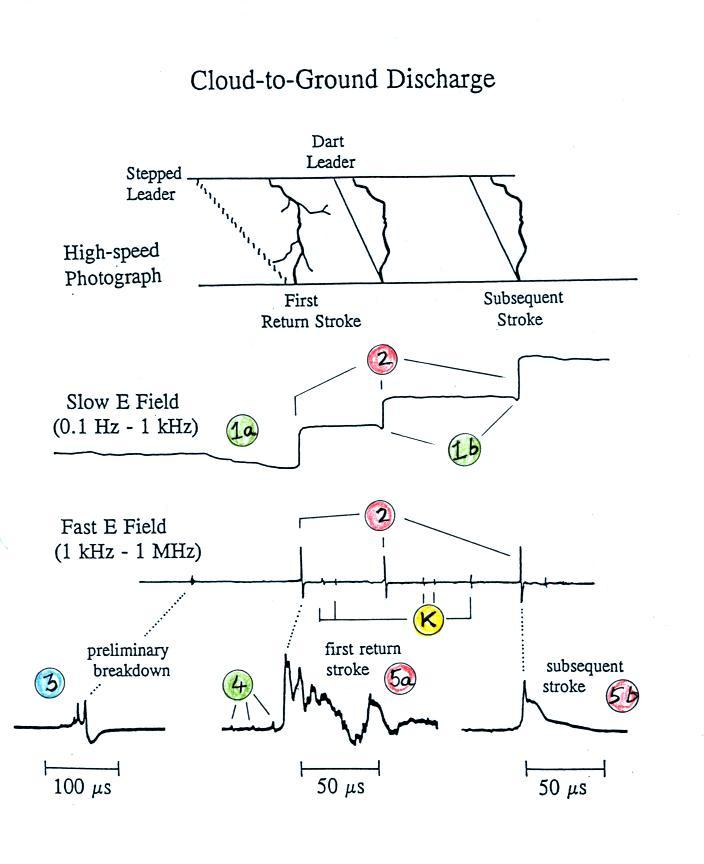
\includegraphics[width=0.8\textwidth]{./images/CG_photo_fields_01.jpg}
			\end{figure}
		\end{minipage}
	\end{tabular} \scriptsize
	선도(leader): 전기장에 의해 구름의 전자가 방출될 때 공기가 이온화되어 형성된 도전로\\
		계단 선도(step leader): 구름 밑면의 전자가 선도 아래로 유입되어 선도 말단의 전위가 증가하고 도전로가 늘어나 이온화가 더 진행되는데, 이와 같이 초기 경로가 보이지 않은 채 지면 쪽으로 확대되는 것을 의미
		화살 선도(dart leader): 첫번째 뇌격 후 추가 뇌격이 뒤따라 오면서 구름 내부 더 높은 지역의 전하를 끌고 오게 됨. 뇌격이 이어질 때마다 화살선도로 시작, 경로를 다시 이온화시키고 구름 전위를 땅으로 이동.\\
\end{frame}




\begin{frame}[t]{구름-지면 번개를 통한 구름의 방전}
	\begin{tabular}{ll}
		\begin{minipage}[t]{0.7\textwidth}\scriptsize
			\begin{figure}[t]
				\includegraphics[trim=50 340 80 50, clip, page=311, width=\textwidth]{\bookfile}
			\end{figure}
		\end{minipage}	
		&
		\begin{minipage}[t]{0.25\textwidth} \scriptsize	
%			물방울이 빙정으로 변하기 시작하면 양이온이 차가운 부분에 모이고, 음이온은 따뜻한 부분에 모임.\\
%			바깥쪽 부터 얼면서 바깥부분이 양전하를 띠고, 안쪽은 음전하가 발달
%			내부가 얼기 시작하면 팽창하여 바깥쪽 껍질이 흩어짐.\\
%			양전하를 띤 가벼운 작은 빙정은 난기류에 상승하고, 음전하를 띤 상대적으로 무거운 물방울은 구름 아랫쪽에 위치
%			거대한 적란운 발생시 전하 분리가 일어나면서 구름의 일부에서는 음전하가 과도하게 발달하고, 다른부분에서는 양전하를 과도하게 얻음.
			
			A: 전하 분리가 구름 안에서 발생함.\\
			구름 밑면 음전하가 지면의 양전하를 유도함.\\
			B: 계단 선도가 공기를 이온화 시켜 좁은 도전로를 형성\\
			C: 밝은 되돌이 뇌격이 경로에 쌓여 있던 전하를 알래로 옮기기 시작함.\\
			D: 되돌이 뇌격이 완성되고, 구름 밑면에서 온 음전하가 아래로 이동함.\\
			E: 화살 선도가 도전로를 재 이온화 시킴. 
			F: 몇 차례 뇌격 후 구름에서 음전하가 빠져나옴.

		\end{minipage}
	\end{tabular}
\end{frame}



\begin{frame}[t]{마이크로 버스트(Microburst)}
	\begin{tabular}{ll}
		\begin{minipage}[t]{0.6\textwidth}\scriptsize
			\begin{figure}[t]
				\includegraphics[trim=50 50 250 450, clip, page=310, width=0.49\textwidth]{\bookfile}
				\includegraphics[trim=350 430 35 110, clip, page=310, width=0.49\textwidth]{\bookfile}
			\end{figure}
		\end{minipage}	
		&
		\begin{minipage}[t]{0.35\textwidth} \scriptsize	
			일부 뇌우 아래에서 하강 버스트(downburst)라는 강한 국지적 하강 기류 발생
			규모가 $4 \rm{~km}$보다 작을 때 마이크로버스트라 부름\\
			증발냉각에 의해 하강 기류가 강화될 때 발생하여 $2 \sim 5$분 지속\\
			차가운 공기는 지표에서 엄청나게 빨라($160 \rm{~km/h}$ 이상) 큰 피해\\
			강한 하강 기류로 인해 이착륙하는 항공기에 큰 위협이 됨 \\
			
			\questionset{마이크로 버스트에서 강한 하강 기류를 만드는 두 가지 요인을 설명하시오.}
			\solutionset{1) 강수가 증발하면서 공기덩이를 냉각시킴. 공기가 냉각될 수록 무거워져서 더욱 빠르게 하강한다.\\
			2) 하강하는 강수가 하강 기류를 강하게 만듬}
			
		
		\end{minipage}
	\end{tabular}
\end{frame}






\begin{frame}[t]{번개}
	\begin{tabular}{ll}
		\begin{minipage}[t]{0.6\textwidth}\scriptsize
			\begin{figure}[t]
				\includegraphics[trim=350 460 40 150, clip, page=312, width=\textwidth]{\bookfile}
			\end{figure}
		\end{minipage}	
		&
		\begin{minipage}[t]{0.35\textwidth} \scriptsize	
			\questionset{그림의 섬광 척도는 3개월치 자료의 합성이다. $6 \sim 8$월, $12 \sim 2$월 중 언제인가?}
			\solutionset{$12 \sim 2$월}

			
		\end{minipage}
	\end{tabular}
\end{frame}




\begin{frame}[t]{천둥}
	\begin{tabular}{ll}
		\begin{minipage}[t]{0.45\textwidth}\scriptsize
			번개에 의해 1초도 안되는 시간에 공기가 $33,000 \rm{^{\circ} C}$ 까지 가열됨. 단기간에 데워짐에 따라 폭발적으로 팽창하여 듣게 되는 음파\\

			광속에 비해 음속은 느리다. 그러므로 번개는 바로 보이지만, 음파는 $330 \rm{~m/s}$의 음속에 따라 전달된다. 거리에 따라 번개 발생후 천둥이 들리는 시간까지의 차이를 측정하면 번개가 친 곳까지의 거리를 추정할 수 있다. 
			
		\end{minipage}	
		&
		\begin{minipage}[t]{0.5\textwidth} \scriptsize	
			\questionset{천둥이 어떻게 만들어지는지 설명하시오.}
			\solutionset{번개에서의 전하 방전은 공기를 가열시키고, 급격히 팽창하게 해서,음파가 형성되어 우리가 듣게 된다. \\
			하지만 번개가 형성된 곳에서 $20\rm{~km}$ 이상 멀어지게 되면 천둥의 소리를 들을 수 없게 되고 이러한 번개를 ‘열번개’라 부른다.}
			
		\end{minipage}
	\end{tabular}
\end{frame}






\section{토네이도}


\begin{frame}[t]{토네이도}
	\begin{tabular}{ll}
		\begin{minipage}[t]{0.45\textwidth}\scriptsize
			\begin{figure}[t]
				\includegraphics[trim=0 390 355 0, clip, page=314, width=0.9\textwidth]{\bookfile}
			\end{figure}
		\end{minipage}	
		&
		\begin{minipage}[t]{0.5\textwidth} \scriptsize	
			평균 지름: $150 \sim 600\rm{~m}$, 평균 이동 속도: $45 \rm{~km/h}$\\
			이동 경로: $26 \rm{~km}$, 이동 방향: NE\\
			지속 시간: 3분 미만 ~ 3시간 이상\\
			평균 풍속: $150 \sim 500 \rm{~km/h}$
			전체 토네이도의 40 \%이상이 봄철에 발생하며, 트위스터(twister), 사이클론(cyclone)이라 부르기도 함.\\
			단기간 지속되는 회전하는 공기 기둥 형태의 파괴적인 바람폭풍\\
			토네이도 내부 기압은 바깥쪽보다 10 \% 이상 낮음\\
			기압이 급속도로 떨어져 공기가 단열 팽창하여 수증기가 응결되어 먼지, 파편과 함께 창백하고 어두운 구름을 형성. 			
		
		\end{minipage}
	\end{tabular}
\end{frame}




\begin{frame}[t]{토네이도}
	\begin{tabular}{ll}
		\begin{minipage}[t]{0.4\textwidth}\scriptsize
			\begin{figure}[t]
				\includegraphics[trim=137 0 0 460, clip, page=314, width=0.8\textwidth]{\bookfile}
				\includegraphics[trim=340 480 50 50, clip, page=315, width=0.9\textwidth]{\bookfile}
			\end{figure}
		\end{minipage}	
		&
		\begin{minipage}[t]{0.55\textwidth} \scriptsize	
			\questionset{토네이도의 풍속이 빠른 이유는 무엇인가?}
			\solutionset{토네이도가 통과해 감에 따라 $40$ 초 동안 $100 \rm{~hPa}$의 현저한 기압 하강을 보임. 매우 큰 기압 경도를 가지고 있기 때문에 풍속이 매우 빠름. \newline}
			
			\questionset{토네이도 형성에 가장 일반적인 대기 조건은 무엇인가?}
			\solutionset{토네이도는 매우 대비되는 기단의 경계인 중위도 저기압의 한랭 전선이나 스콜선을 따라 형성되거나, 초대형 세포 뇌우와 관련되어 형성됨.}
			
		\end{minipage}
	\end{tabular}
\end{frame}




\begin{frame}[t]{다중 소용돌이 토네이도(multiple-vortex tornado)}
	\begin{tabular}{ll}
		\begin{minipage}[t]{0.45\textwidth}\scriptsize
			\begin{figure}[t]
				\includegraphics[trim=40 350 350 150, clip, page=315, width=\textwidth]{\bookfile}

			\end{figure}
		\end{minipage}	
		&
		\begin{minipage}[t]{0.5\textwidth} \scriptsize	
			강력한 토네이도는 큰 토네이도의 중심 주위를 궤도를 그리며 도는 흡입소용돌이(suction vortex)라 불리는 작지만 강력한 소용돌이를 내포.\\
			이런 경우를 다중 소용돌이 토네이도(multiple-vortex tornado)로 분류한다.\\
			흡입소용돌이의 지름은 약 $10\rm{~m}$, 지속시간은 $1$ 분 이내
			
			
		\end{minipage}
	\end{tabular}
\end{frame}






\section{토네이도의 발달과 발생}



\begin{frame}[t]{토네이도의 생성과 발달}
	\begin{tabular}{ll}
		\begin{minipage}[t]{0.65\textwidth}\scriptsize
			\begin{figure}[t]
				\includegraphics[trim=50 430 50 50, clip, page=316, width=\textwidth]{\bookfile}
			\end{figure}
		\end{minipage}	
		&
		\begin{minipage}[t]{0.3\textwidth} \scriptsize	
			상층 바람이 지상 바람보다 강해 수평축 방향 회전 존재 (연직바람시어 존재)\\
			뇌우가 형성되며 상승 기류가 수평으로 회전하는 공기를 수직으로 기울임\\
			회전하는 공기의 연직 원기둥인 중규모 저기압이 형성\\
			수평으로 좁아지고, 회전 속도 증가하고, 벽구름이 형성되고, 깔대기 구름이 나와 지면 접촉
			
		\end{minipage}
	\end{tabular}
\end{frame}




\begin{frame}[t]{토네이도의 특징}
	\begin{tabular}{ll}
		\begin{minipage}[t]{0.55\textwidth}\scriptsize
			\begin{figure}[t]
				\includegraphics[trim=280 50 40 530, clip, page=316, width=\textwidth]{\bookfile}
			\end{figure}
		\end{minipage}	
		&
		\begin{minipage}[t]{0.40\textwidth} \scriptsize	
			\questionset{토네이도 시즌은 언제이며, 그 시기에 발생하는 이유는 무엇인가?}
			\solutionset{봄과 초여름(4월 $\sim$ 7월)이 토네이도의 활동이 가장 활발한 시기이다. \\
			이는 온도차이가 클수록 강한 폭풍이 발달하는데, 중위도 저기압과 관련된 기단들이 봄철에 가장 큰 온도 차이를 가지고 있기 때문이다.}
			
		
		\end{minipage}
	\end{tabular}
\end{frame}




\begin{frame}[t]{토네이도의 특징}
	\begin{tabular}{ll}
		\begin{minipage}[t]{0.45\textwidth}\scriptsize
			\begin{figure}[t]
				\includegraphics[trim=350 0 50 390, clip, page=317, width=0.8\textwidth]{\bookfile}
			\end{figure}
		\end{minipage}	
		&
		\begin{minipage}[t]{0.5\textwidth} \scriptsize	
			\questionset{토네이도의 이동방향을 설명하시오.}
			\solutionset{토네이도는 한랭 전선 앞의 강한 바람에 의해 이동하므로, 대부분의 토네이도가 남서에서 북동 방향으로 이동함.}
						
		\end{minipage}
	\end{tabular}
\end{frame}




\begin{frame}[t]{토네이도의 극한치}
	\begin{tabular}{ll}
		\begin{minipage}[t]{0.9\textwidth}\scriptsize
			\begin{figure}[t]
				\includegraphics[trim=40 500 40 50, clip, page=318, width=\textwidth]{\bookfile}
			\end{figure}
		\end{minipage}	
		&
		\begin{minipage}[t]{0.5\textwidth} \scriptsize	
			
			
		\end{minipage}
	\end{tabular}
\end{frame}




\begin{frame}[t]{토네이도}
	\begin{tabular}{ll}
		\begin{minipage}[t]{0.45\textwidth}\scriptsize
			\begin{figure}[t]
				\includegraphics[trim=0 520 255 0, clip, page=317, width=\textwidth]{\bookfile}
			\end{figure}
			November tornado
		\end{minipage}	
		&
		\begin{minipage}[t]{0.5\textwidth} \scriptsize	
			\begin{figure}[t]
				\includegraphics[trim=250 30 50 420, clip, page=318, width=\textwidth]{\bookfile}
			\end{figure}
			
		\end{minipage}
	\end{tabular}
\end{frame}






\section{토네이도의 파괴와 토네이도 예보}



\begin{frame}[t]{토네이도 강도}
	\begin{tabular}{ll}
		\begin{minipage}[t]{0.45\textwidth}\scriptsize
			\begin{figure}[t]
				\includegraphics[trim=50 430 330 50, clip, page=320, width=\textwidth]{\bookfile}
			\end{figure}
		\end{minipage}	
		&
		\begin{minipage}[t]{0.5\textwidth} \scriptsize	
			\begin{figure}[t]
				\includegraphics[trim=50 490 350 50, clip, page=321, width=0.8\textwidth]{\bookfile}
			\end{figure}
			강도: 증보 후지타 척도(Enhanced Fujita scale)로 폭풍에 의한 가장 큰 피해를 기준으로 등급 매김
			
			
		\end{minipage}
	\end{tabular}
\end{frame}




\begin{frame}[t]{토네이도의 흔적}
	\begin{tabular}{ll}
		\begin{minipage}[t]{0.9\textwidth}\scriptsize
			\begin{figure}[t]
				\includegraphics[trim=50 55 30 530, clip, page=322, width=\textwidth]{\bookfile}
			\end{figure}
		\end{minipage}	
		&
		\begin{minipage}[t]{0.05\textwidth} \scriptsize	
			
			
		\end{minipage}
	\end{tabular}
\end{frame}




\begin{frame}[t]{도플러 레이더}
	\begin{tabular}{ll}
		\begin{minipage}[t]{0.9\textwidth}\scriptsize
			\begin{figure}[t]
				\includegraphics[trim=30 30 50 575, clip, page=324, width=\textwidth]{\bookfile}
			\end{figure}
		\end{minipage}	
		&
		\begin{minipage}[t]{0.05\textwidth} \scriptsize	
			
			
		\end{minipage}
	\end{tabular}
\end{frame}




\begin{frame}[t]{도플러 레이더}
	\begin{tabular}{ll}
		\begin{minipage}[t]{0.55\textwidth}\scriptsize
			\begin{figure}[t]
				\includegraphics[trim=30 570 345 50, clip, page=325, width=\textwidth]{\bookfile}
			\end{figure}
		\end{minipage}	
		&
		\begin{minipage}[t]{0.4\textwidth} \scriptsize	
			\begin{figure}[t]
				\includegraphics[trim=350 350 50 50, clip, page=324, width=\textwidth]{\bookfile}
			\end{figure}
			
		\end{minipage}
	\end{tabular}
\end{frame}
